% Intended LaTeX compiler: pdflatex
\documentclass[10pt,a4paper,UTF8]{article}
\usepackage{zclorg}
\usepackage{tikztheorem}
\author{张朝龙}
\date{}
\title{如何管理自己的自由时间}
\hypersetup{
 pdfauthor={张朝龙},
 pdftitle={如何管理自己的自由时间},
 pdfkeywords={reading},
 pdfsubject={},
 pdfcreator={Emacs 25.0.50.1 (Org mode 9.0.6)},
 pdflang={English}}
\begin{document}

\maketitle
\tableofcontents
\titlepic{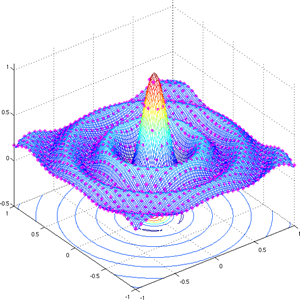
\includegraphics[scale=0.25]{../../img/sinc.PNG}}

\section{背景}
\label{sec:org9e4c61b}
最近小孩出生,生活一下子忙碌起来,自由时间永远处于奢侈品状态,更别说抽出大量的时间去充电。直到我再次看到TED 的演讲\href{http://open.163.com/movie/2016/12/I/B/MC82BCQAN\_MC8U8L3IB.html}{《如何管理自己的自由时间》} 。稍有感悟,记录如下。

\section{时间永远有的}
\label{sec:orgc645955}

时间永远都是有的,只不过看你愿意不愿意投入。劳拉在演讲中举了一个例子:一个女主人家的热水器管子爆裂,她必须处理这个事情,结果最后统计她在这一周足足多了7个小时来做这个事情。这说明什么,以前她也可以多出7个小时来。之所以没有,是因为事情不够重要!

结论一:我没有时间,不是真的没有时间,而是这件事情不那么重要。那么,为什么我不主动去选择呢?我可以选择在地铁上阅读一本书的一个章节而不是阅读手机上的八卦新闻;我可以在周末观看学习新领域的公开课,而不是追剧;我可以抽出半个小时去跑步,而不是犹豫到底要不要锻炼。我的生活,就是我的选择。
\section{自由时间和理想生活的逻辑}
\label{sec:org7d566c7}


通过这个演讲,我还知道自己犯了另外一个逻辑错误:通常,我总以为有了自由时间我就可以过上理想的生活,其实相反;应该是,我选择去过理想的生活,我才会有自由时间。原来,我一直过一种本末倒置的生活。或者说,我一直过一种没有目标的生活。拥有自由时间根本不是目标,而是理想生活的副产品。我选择去跑步,于是我有了跑步的自由时间;我选择阅读,于是我有了阅读的时间;我选择陪伴家人,于是我有了陪伴家人的时间。跑步,阅读和陪伴家人这些事情之所以在之前没有时间做,是因为我根本就没有把他们当做理想生活的一部分!多么可怕难道我不想过这样的生活嗯?是的!按照之前我的时间支出确实如此。我总是欺骗自己,认为这些活动是有了自由时间才可以展开的。

结论二:我们选择了什么样的生活,我们才有什么样的时间。选择生活中如何投入时间是一件相对有自由选择权的事情,比如你可以选择早上早餐快一点,而不是磨磨蹭蹭,这样就有时间去跑步;比如可以选择在通勤地铁上拿出多看阅读一本书,而不是掏出iphone刷朋友圈或者知乎;比如可以拒绝无聊的聚会,选择陪伴家人\ldots{}\ldots{}

\section{先定目标再安排时间}
\label{sec:orga483a8e}


需要常常提醒自己这些道理。没有目标,时间都会在大量的无意义的琐事中虚度。这些琐事不能为人生的成长提供任何营养。我需要经常责问自己:为什么这些琐事居然会成为选择?是不是忘记了目标?回首毕业之后三年工作经历,第一年还如人所愿,到后来感觉自己过的急匆匆的,如同浮萍被激流挟着前进。很多事情做起来都不是本人所愿。公司的要求过于急躁,无法静心做事。静心做事之后发现资源都被糙猛快占据。要我选择糙猛快,比登天还难。我希望成为一个工匠,精益求精的工匠。做一件事情应该如同打磨一件玉器一样,单是过程就应该足以令人愉悦。

当我发现,公司能够提供的环境不能和自己的目标匹配时,我选择了妥协,变成浮萍,被涛涛洪流挟了去。为什么?我被这份工资给绑架了,失去了改变的勇气,变成了温水的青蛙,慢慢失去知觉,等着被清理。

既然我已知晓原因,为什么不选择改变呢?是的,改变是痛苦的。但是,我必须警醒自己,不改变更痛苦。人总是趋利避害,选择更小的痛苦,然后慢慢的被绑架再无挣扎之力。

\section{我选故我在}
\label{sec:org5bafae9}


所做事情必须与目标一致,自由时间只是个副产品。我的选择构成了我的生活,而不是那些安排在自由时间的活动。
\end{document}
